\section{Approach}
\label{sec:method}

%Inspired by the match-LSTM with word-by-word attention \cite{wang2016learning}, 
We propose an attention-based neural network model for QA matching 
in multi-turn dialogues between two parties. 
Given a Q-NQ pair with its distance and history, 
the model consists of four components (shown in Figure \ref{fig:model1}): 
\textit{Sentence Encoder} transforms the natural language turns into 
sentence-level embeddings. \textit{Mutual Attention} combines history turns 
based on two simultaneous attention mechanisms in an interleaving way. 
\textit{Match-LSTM} is used to compare the processed sentence pair word by word. 
\textit{Prediction Layer} incorporates the distance information 
and calculates the alignment probability. After calculating the probability for 
all Q-NQ pairs in a dialogue, a \textit{greedy matching algorithm} is employed to
match each NQ to zero or one Q.
 %\textit{History Adder} consists of two parallel attention mechanisms to add history information into the pairwise model. 

%\KZ{Restructure fig 2 to reflect the four components in the archi. Mention fig 2 
%in the preamble of the section.}

\begin{figure*}
	\centering
	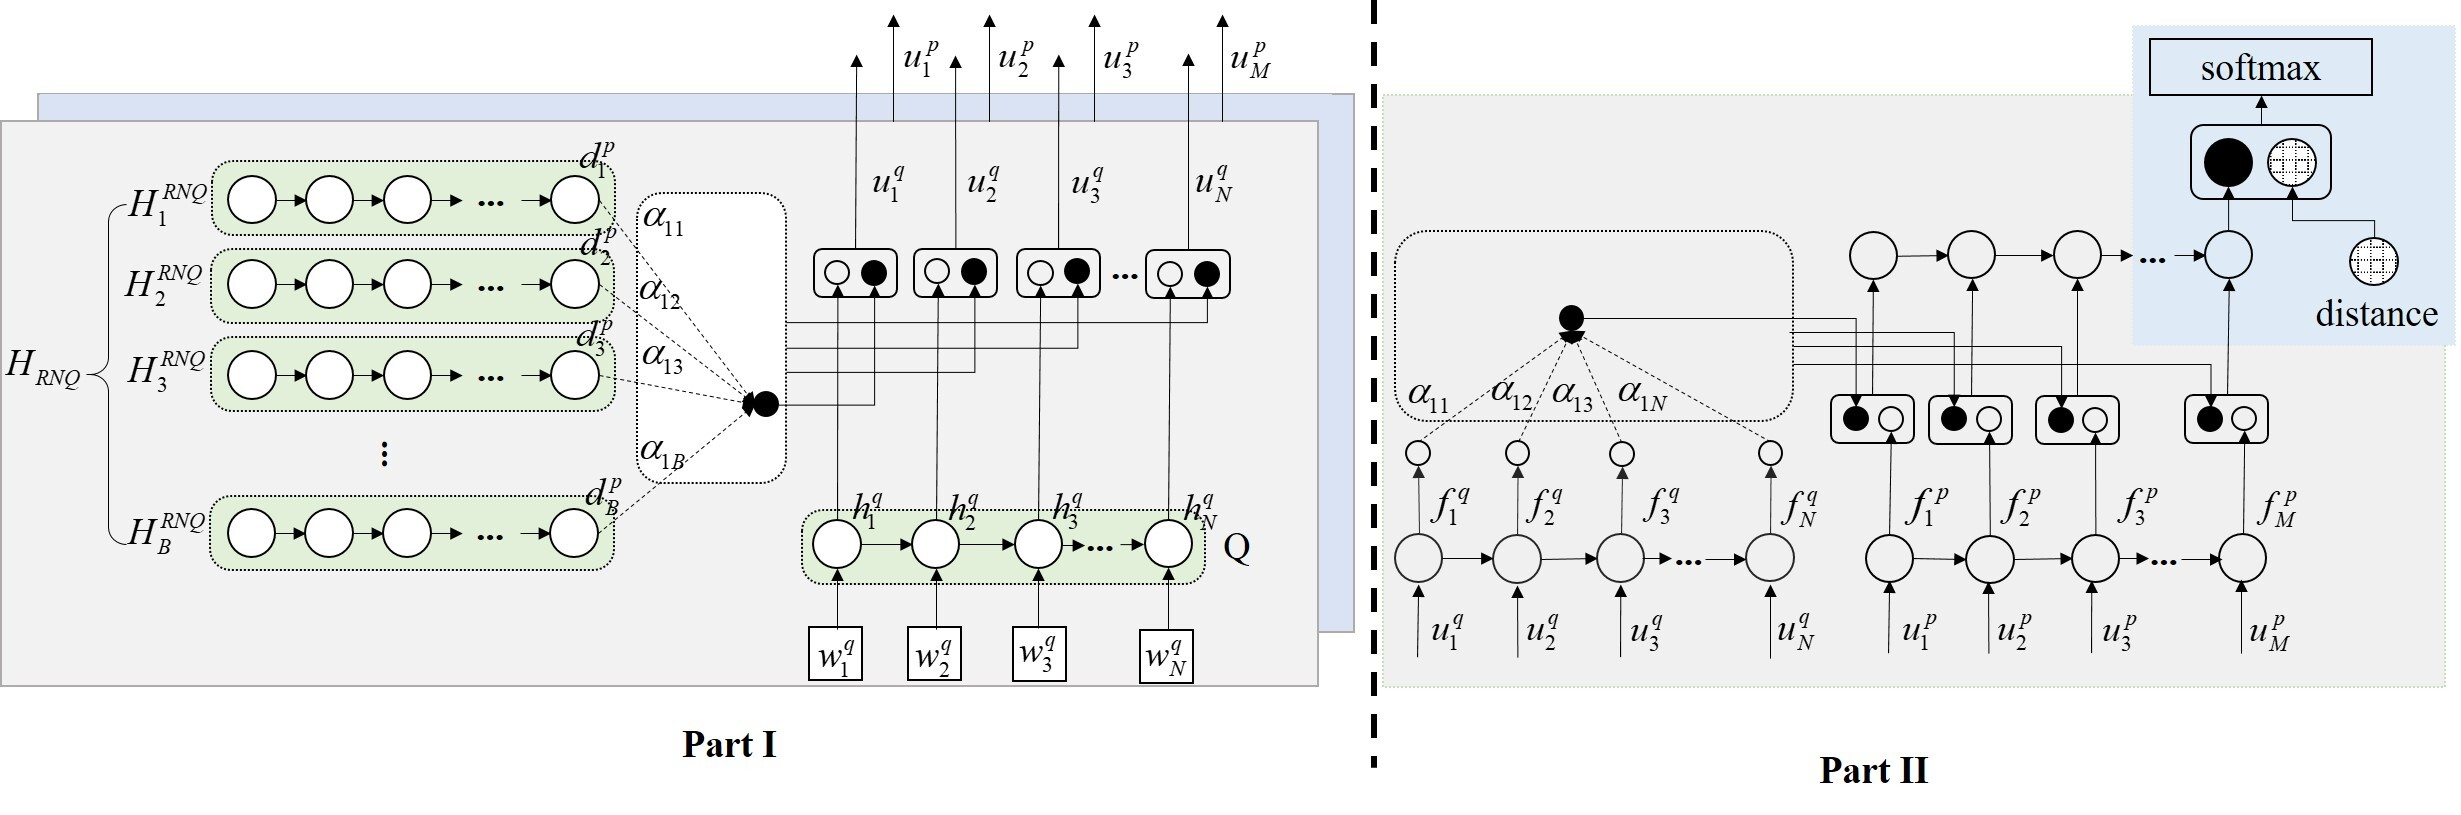
\includegraphics[scale=0.40]{pictures/figure3_new.pdf}
	\caption{The architecture of the proposed match-LSTM based model with parallel attention mechanisms. \textbf{Part I:} Sentence Encoder and Mutual Attention. Front plate
(gray) shows the encoding of Q, while the back plate (blue) includes the encoding of a NQ.
The green part is Sentence Encoder and the rest is Mutual Attention. \textbf{Part II:} Match-LSTM and Prediction Layer. The gray part is Match-LSTM and the blue part is Prediction Layer.}
	
	\label{fig:model1}
\end{figure*}

\subsection{Sentence Encoder}
\label{sec:sentence-encoder}

Given an input turn as a sequence of words in natural language, we generate a neural representation using an LSTM \cite{gers1999learning}. The input layer consists of pretrained word embeddings of the words which are fed into a single hidden layer. The output of all the hidden states or the last hidden state can both be regarded as the sentence-level embedding for this turn.

With the sentence encoder, we can get the neural representations for a Q-NQ pair and its history as follows:
\begin{equation}
\begin{aligned}
Q&=\{h_i^q\}_{i=1}^{N}\\
NQ&= \{h_i^p\}_{i=1}^{M}\\
H_{RQ}&=\{d_t^q\}_{t=1}^{A}\\
H_{RNQ}&=\{d_t^p\}_{t=1}^{B}\\
\end{aligned}
\end{equation}
%\KZ{Explain what is N, M, q, i, t, all the parameters, and what are h and d?}
where the number of words in $Q$ and $NQ$ are $N$ and $M$ respectively. $h^i$ represents the hidden state of each word. $H_{RQ}$ and $H_{RNQ}$ represents the history turns with the same role label as $Q$ and $NQ$ respectively. $A$ and $B$ are the number of turns in each $H_{RQ}$ and $H_{RNQ}$ respectively, and $d_t$ is the last hidden state of each turn. Superscripts $p$ and $q$ are used to distinguish $Q$ and $NQ$. Here, we divide the history turns into 
two parts to support for the idea of mutual attentions between Q and NQ
in the following subsection.

The intuition for using different granularity of sentence embeddings is that we hope to 
keep more information for more important turns. Therefore, in order to calculate 
the matching score between a Q-NQ pair, we preserve all the hidden states for Q and NQ. 
The last hidden state of each turn in history is used to provide auxiliary information.

%We name the participant who raised the question utterance as $role_Q (RQ)$. The other participant who raised the non-question utterance is named as $role_P (RP)$. After converting each word to embedding, $H_{RQ}=\{ \{w_{1t}^{q}\}_{t=1}^{N_1}, \{w_{2t}^{q}\}_{t=1}^{N_2}... ,\{w_{At}^{q}\}_{t=1}^{N_A} \}$ and $H_{RP}=\{ \{w_{1t}^{p}\}_{t=1}^{M_1}, \{w_{2t}^{p}\}_{t=1}^{M_2}... ,\{w_{Bt}^{p}\}_{t=1}^{M_B} \}$.

 %We then use one-layer LSTM model proposed by \cite{gers1999learning} to obtain the sentence embedding. Specifically, we use all the hidden states output from LSTM to encode $Q$ ($\{h_t^q\}_{t=1}^{N}$) and $NQ$ ($ \{h_t^p\}_{t=1}^{M}$), but use the last state of LSTM to encode several history sentences in $H_{RQ}$ ($\{d_t^q\}_{t=1}^{A}$) and $H_{RP}$ ($\{d_t^p\}_{t=1}^{B}$).



\subsection{Mutual Attention to the History}
\label{sec:mutual attention}
To improve the prediction for each Q-NQ pair, 
naturally we take advantage of the dialogue context, 
especially the turns between Q and NQ. 
This idea comes from two considerations: i) if Q has been partially answered 
by another NQ between the current pair of Q and NQ, then we should further explore 
whether the current NQ is a supplementary answer; ii) if there exists another Q which is closer 
to the NQ in both distance and semantics, the probability of matching 
the current Q-NQ pair should reduce. In a word, 
if the model can capture these intuitions, it's more likely to match 
the LQAs such as \{U2,U10\}.

Besides, it should be noted that the question and matching answer should
definitely be uttered by different parties. 
In other words, the QA relations in a dialogue is focusing 
on the process of narrowing down the information gap between two parties, 
where the information interaction between parties is critical. 
So, we further divide the history into two parts: 
$H_{RQ}$ and $H_{RNQ}$ by different role labels as mentioned above. 
$Q$ is expected to interact with $H_{RNQ}$ while $NQ$ is expected to interact with $H_{RQ}$.

Borrowing the idea from Wang et al. \cite{wang2017gated}, we use two attention mechanisms to incorporate the history information into Q and NQ individually in a unified manner. For example, when dealing with the Q-NQ pair $\{U2,U10\}$, $H_{RQ}=\{U3,U7,U9\}$ and $H_{RNQ}=\{U4,U5,U6,U8\}$. The neural representation of $U2$ attends to $H_{RNQ}$ and $U10$ attends to $H_{RQ}$ simultaneously.
In other words, Q and NQ ``mutually'' attend to each other's history. Mathematically, as for $Q$ and $H_{RNQ}$: the $Q$ containing historical information can be obtained  via soft alignment of words in the question $Q=[h^q_1,h^q_2,...,h^q_N]$ and history turns $H_{RNQ}=\{d^p_1,d^p_2,...,d^p_B\}$ as follows (see Part I in Figure \ref{fig:model1}):

\begin{equation}
u^q_i=[h^q_i,c^q_i]
\end{equation}
where $c^q_i=att(h^q_i,H_{RNQ})$ is an attention-pooling vector of the whole history($H_{RNQ}$),
, and $v$ and $W$ are the weights:
\begin{equation}
\begin{aligned}
s^i_j&=v^Ttanh(W_Qh^q_i+W_Hd^p_j)\\
a^i_k&=exp(s^i_k)/\sum_{j=1}^Bexp(s^i_j)\\
c^q_i&=\sum_{k=1}^Ba^i_kd^p_k
\end{aligned}
\end{equation}
Each word representation in $Q$ dynamically incorporates aggregated matching information from the history $H_{RNQ}$. 

The final representations of the question and the non-question after
mutual attention are $Q^\prime=[u^q_1,u^q_2,...,u^q_N]$ and 
$NQ^\prime=[u^p_1,u^p_2,...,u^p_M]$. Each word vector
in $Q^\prime$ and $NQ^\prime$ not only represents the original sentence meaning 
but also contains dialogue context. The effects of 
different choices of turns in history and the ways of aggregating the 
history will be discussed later.


\subsection{Match-LSTM}
We follow the work of Wang and Jiang~\cite{wang2016learning} 
and adopt match-LSTM to capture the features between the 
processed $Q^\prime$ and $NQ^\prime$ word by word.

As Part II of \figref{fig:model1} shows,
a one-layer LSTM is used to encode the representations with mutual attention for 
questions and non-questions. 
We thus obtain $Q^{\prime\prime}=\{f^q_i\}_{i=1}^{N}$ and 
$NQ^{\prime\prime}=\{f^p_i\}_{i=1}^{M}$. 
When encoding the non-question, we introduce a series of attention-weighted 
combinations of the hidden states of the question, where each combination is for a particular word in the non-question. The sentence-pair representation $P=\{p_i\}_{i=1}^{M}$ is calculated with attention mechanism as follows. 

\begin{equation}
    p_i=LSTM(p_{i-1},[f^p_i,c_i])
\end{equation}
where $c_i=att(Q,f^p_i,p_{i-1})$ is an attention-pooling vector of the whole question($Q$):
%\begin{center}
\begin{equation}
\begin{aligned}
s^i_j&=v^Ttanh(W_{NQ}f^p_i+W_Qf^q_j+W_pp_{i-1})\\
a^i_k&=exp(s^i_k)/\sum_{j=1}^Nexp(s^i_j)\\
c_i&=\sum_{k=1}^Na^i_kf^q_k
\end{aligned}
%\end{gather}
\end{equation}
%\end{center}

Finally, we use $p_M$ to represent the whole Q-NQ pair which is used for predicting the final result.

\subsection{Prediction Layer }
At the last step, we use a fully-connected (FC) layer with softmax to do binary classification, which indicates whether this pair of utterance has QA relation.

Driven by the intuition that distance is a critical feature 
for matching QA pairs, %(which will be shown in Section \ref{sec:results}), 
we explicitly add the distance at the end of our model to 
preserve its effectiveness. The distance $d$ is defined as 
a 10-dimensional one-hot vector, where the position of 
1 is equal to the distance. For example, if the distance is 4, then
the 4th dimension of the vector is set to 1. If $d\geq 10$, then the 10th
dimension is set to 1.

Finally, the probability is calculated as follows:
\begin{equation}
\begin{aligned}
FC&=W[p_M,d]+b\\
P(Q,NQ)&=Softmax(FC)
\end{aligned}
\end{equation}

In sum, the input of our model is a Q and NQ with associated information (history and distance), and the output of model is the probability of being \textit{True} or \textit{False} which indicates if the Q is the matched question of the NQ. Hence, the loss function is the cross entropy between the predicted probability $P(Q,NQ)$ and the ground truth. The model can be seen as a binary classification model and all the parameters are trained altogether except the pretrained word embeddings.

\subsection{Greedy QA Matching}

Based on the trained model, every NQ now has a matching probability with every Q 
before it in the dialogue sequence. The greedy algorithm matches the NQ with the
Q with maximum probability if that probability exceeds 0.5.
The threshold is set to 0.5 because our model is actually a two-class classifier.
%The final prediction is chosen as follows:
%\begin{equation}
%Q^\star=\left\{
%\begin{aligned}
%\arg\max_{Q\in \Omega}&P(Q,NQ)  &P(Q^\star,NQ)\geq 0.5 \\
% \varnothing&  &otherwise \\
%\end{aligned}
%\right.
%\end{equation}




% Since it is a two-class classification problem, we naturally choose 0.5 as our threshold. We simply choose the $Q$ with the max probability.


%if $p>0.5$, then we say there is a QA relation between this NQ and associated $Q_{i}$, and this NQ will be labeled as $A_i$. Otherwise, the NQ will be predicted as $O$. 







